\documentclass[11pt,a4paper]{article}

\usepackage{fontspec}
\usepackage[a4paper,margin=2.1cm]{geometry}
\usepackage{booktabs}
\usepackage{tabularx}
\usepackage{array}
\usepackage[table]{xcolor}
\usepackage{enumitem}
\usepackage{listings}
\usepackage{titlesec}
\usepackage{caption}
\usepackage{float}
\usepackage{needspace}
\usepackage{tikz}
\usetikzlibrary{positioning,fit,arrows.meta,backgrounds,calc}
\usepackage[hidelinks]{hyperref}

\setmainfont{texgyrepagella}[Extension=.otf, UprightFont=*-regular, BoldFont=*-bold, ItalicFont=*-italic, BoldItalicFont=*-bolditalic]
\setsansfont{texgyreheros}[Extension=.otf, UprightFont=*-regular, BoldFont=*-bold, ItalicFont=*-italic, BoldItalicFont=*-bolditalic]

\definecolor{accent}{HTML}{1F4E79}
\definecolor{codebg}{HTML}{F6F7F9}

\titleformat{\section}{\sffamily\large\bfseries\color{accent}}{\thesection}{0.6em}{}
\titleformat{\subsection}{\sffamily\normalsize\bfseries}{\thesubsection}{0.6em}{}
\titlespacing*{\section}{0pt}{1.0em}{0.35em}
\titlespacing*{\subsection}{0pt}{0.7em}{0.25em}

\setlength{\parindent}{0pt}
\setlength{\parskip}{0.4em}
\setlength{\emergencystretch}{3em}
\renewcommand{\arraystretch}{1.15}
\newcolumntype{Y}{>{\raggedright\arraybackslash}X}
\newcolumntype{P}[1]{>{\raggedright\arraybackslash}p{#1}}
\setlist{itemsep=0.05em, topsep=0.15em}
\captionsetup{font=small, labelfont=bf, skip=4pt}
\pagestyle{plain}

\lstset{basicstyle=\ttfamily\footnotesize, backgroundcolor=\color{codebg},
  frame=single, rulecolor=\color{gray!40}, framesep=4pt, xleftmargin=6pt, xrightmargin=6pt,
  columns=fullflexible, keepspaces=true, breaklines=true, showstringspaces=false,
  comment=[l]{//}, commentstyle=\color{gray}\itshape}

\newcommand{\code}[1]{\texttt{#1}}
\newcommand{\ph}[1]{\textit{\color{gray}[#1]}}

% Figure styles
\tikzset{
  box/.style={draw, rounded corners=2pt, align=center, font=\footnotesize,
              minimum height=1.05cm, inner sep=4pt, fill=white},
  zone/.style={draw=gray!70, dashed, rounded corners=4pt, inner sep=7pt},
  zonelabel/.style={font=\scriptsize\sffamily, text=gray!40!black},
  lbl/.style={font=\scriptsize, fill=white, inner sep=1.5pt},
  plain/.style={-{Stealth[length=2mm]}, thin},
  ctrl/.style={-{Stealth[length=2mm]}, dashed, gray!60!black},
  data/.style={-{Stealth[length=2.4mm]}, line width=1.2pt, accent},
  sched/.style={-{Stealth[length=2mm]}, densely dotted, thick},
}

\begin{document}

% ---------------------------------------------------------------------------
\begin{center}
  {\sffamily\small\color{accent} PROJECT PROPOSAL}\\[3pt]
  {\sffamily\bfseries\Large Enforcing Booked Slots on Research-Lab PCs\\[2pt]
   with a Self-Hosted Headscale Server}\\[5pt]
  {\small A 15-machine pilot}\\[6pt]
  {\small \textbf{Prepared by} Zamiul Rashid, Akid Anis and Tanzim Ahmed}\\[2pt]
  {\small \textbf{Supervisor} Md.\ Golam Rabiul Alam \quad·\quad
   \textbf{Co-supervisor} Mollah Md.\ Saif \quad·\quad October 2026}
\end{center}
\vspace{-0.4em}
\suppressfloats[t]

\textbf{Summary.} Every thesis group already has booked slots on our lab PCs,
but nothing enforces them. Groups work remotely through AnyDesk, and anyone with
a PC's AnyDesk details can connect at any time. We have built a system that
enforces the slots, and tested it. A self-hosted Headscale server (an
open-source control server for the Tailscale/WireGuard VPN) admits only
students who sign in with their BRACU Google account. The lab's weekly routine
stays in a Google Sheet. Our slot system, \textbf{labslots}, reads it every 30
seconds; at each slot change it rewrites the network policy and switches the
PC to the incoming group's account, so only the group in its slot can reach its
PC. Every login to a lab PC uses Tailscale SSH, so there are no keys or
passwords to hand out or take back. The system already runs on our own hardware
with three lab PCs. In a test with 871 simulated devices on a 4-core server,
every slot change took effect within 20 seconds, and none of 2,956 login checks
got in where it should not have. For a 15-PC pilot on campus we need
\textbf{one public IP address, one domain name under \code{bracu.ac.bd}, two
inbound ports (three with HTTP) and a lab email account} (Section~\ref{sec:uni}).

% ---------------------------------------------------------------------------
\section{Background and Goals}

Each thesis group is assigned two 12-hour slots per week on a lab PC and works
remotely through AnyDesk. The slots exist only on paper. AnyDesk connects
through AnyDesk's own servers, so anyone who knows a PC's ID and password can
connect whenever they like. That person can stop another group's training run,
change its files or take over its desktop, and nobody can tell afterwards who
did it. A group has one to five students, and students often use more than one
device. Physical access stays under the lab's existing rules. The pilot aims
to:

\begin{enumerate}[leftmargin=1.6em]
  \item Enforce the slots: during a slot only that group can reach its PC
        remotely; outside it, nobody except the lab admins.
  \item Run Headscale and the slot system on one machine in the lab, reachable
        through one public IP address and one domain name.
  \item Enroll 15 Linux lab PCs, each registered once as a lab-owned machine.
  \item Let students sign in with their BRACU Google account, so the lab keeps
        no passwords.
  \item Switch access automatically at every slot change, and record every
        change and every enforcement step.
  \item Keep the schedule where the lab already keeps it, a Google Sheet, and
        take group enrollments through our own page instead of a Google Form.
  \item Measure reliability and load before any wider roll-out.
\end{enumerate}

\newpage
% ---------------------------------------------------------------------------
\section{Options Considered: Why Headscale}

Table~\ref{tab:why} compares the main ways to give students remote access to lab PCs.

\begin{table}[H]
\centering\footnotesize
\renewcommand{\arraystretch}{1.05}
\caption{Options for remote access.}
\label{tab:why}
\begin{tabularx}{\textwidth}{P{3.0cm}P{3.3cm}Y}
\toprule
Option & Control and data path & Fit for slot-based lab access \\
\midrule
Current setup: AnyDesk only & AnyDesk's servers & No slot enforcement: anyone with a PC's ID and password can connect at any time, and there is no record of who did \\
SSH port-forwarding or a bastion host & Ports opened on campus; SSH exposed to the internet & Needs more than one IP and port from IT; open to brute-force attempts; slots enforced only on each PC \\
Plain WireGuard (hub) & Our server; all traffic through the hub & No NAT traversal; keys and firewall rules managed by hand for every device \\
Tailscale (hosted) & Tailscale Inc.\ (off campus); direct P2P & Can share a device into a group's own tailnet by email. The free plan covers 6 users; Standard costs \$8 per user per month. The control plane and user data stay off campus \\
NetBird (self-hosted) & Ours; direct P2P & Capable, but several services to run (management, signal, relay, dashboard, identity provider) and its own clients \\
\textbf{Headscale} (chosen) & \textbf{Ours; direct P2P} & One binary plus SQLite, official Tailscale clients, free (BSD-3). The policy is one document we regenerate and load through its API at every slot change \\
\bottomrule
\end{tabularx}
\end{table}

% ---------------------------------------------------------------------------
\section{System Architecture}

The design separates a \textbf{control plane} from a \textbf{data plane}
(Figure~\ref{fig:arch}). Headscale is an open-source reimplementation of
Tailscale's coordination server that works with the official Tailscale
clients. It registers devices, hands out tailnet addresses and keys, and
pushes each device a peer list filtered by the access policy. It never
carries user traffic. The data plane is WireGuard, running directly between
the student's laptop and the lab PC. Next to Headscale runs labslots: a
website (the \emph{hub}) and a \emph{slot agent} that enforces the schedule.

\begin{figure}[t]
\centering
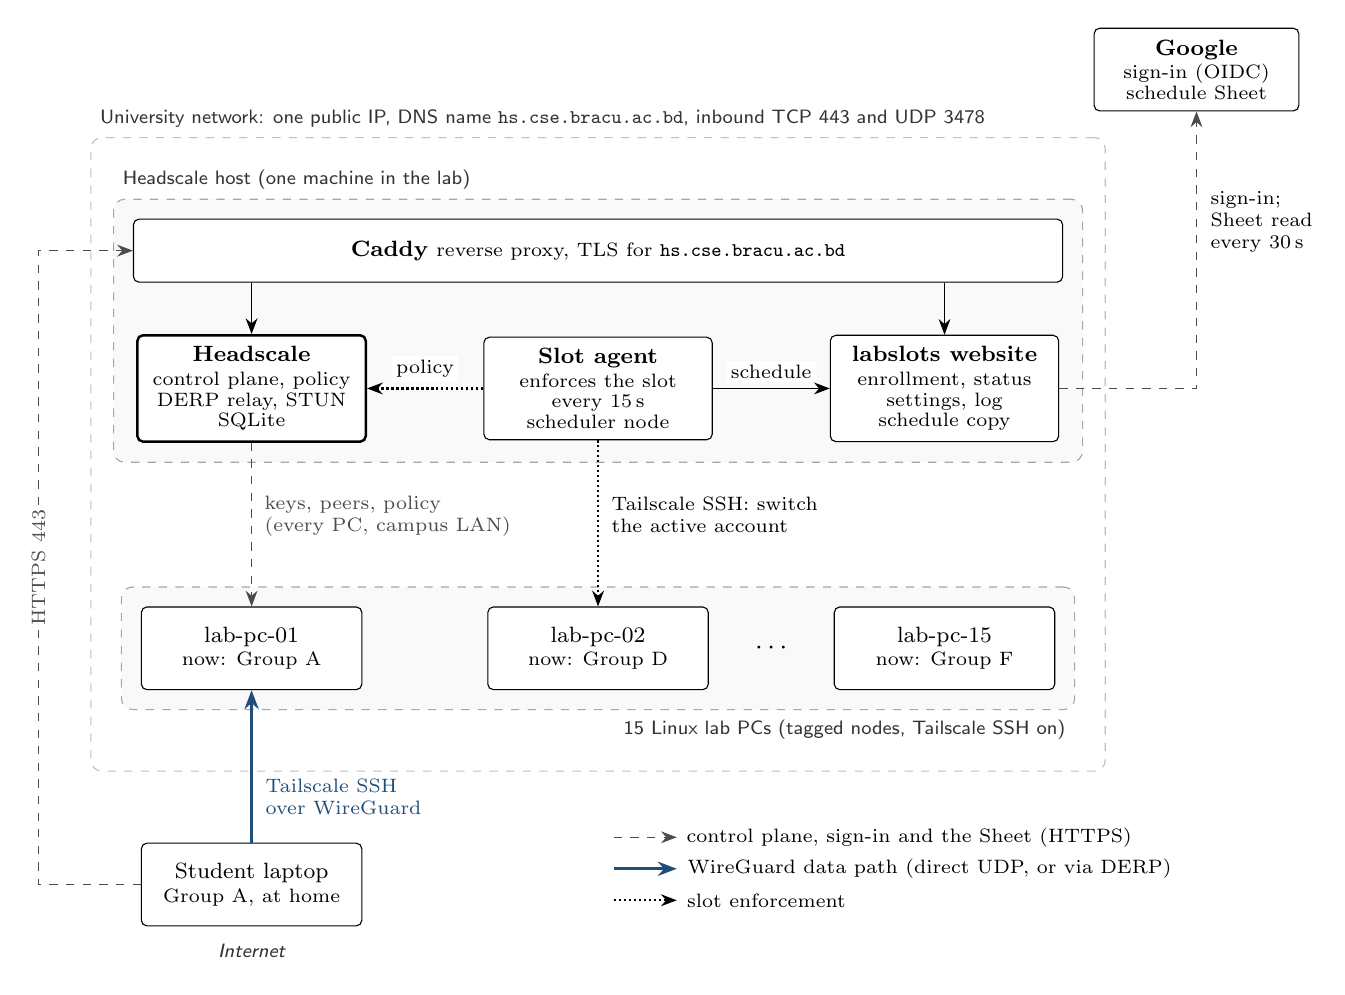
\begin{tikzpicture}
  % ---- Headscale host ----
  \node[box, minimum width=11.8cm, minimum height=0.8cm] (cd) at (4.4,1.75)
       {\textbf{Caddy}\ \scriptsize reverse proxy, TLS for \texttt{hs.cse.bracu.ac.bd}};
  \node[box, minimum width=2.9cm, line width=0.9pt] (hs) at (0,0)
       {\textbf{Headscale}\\[-1pt]\scriptsize control plane, policy\\[-2pt]\scriptsize DERP relay, STUN\\[-2pt]\scriptsize SQLite};
  \node[box, minimum width=2.9cm] (sc) at (4.4,0)
       {\textbf{Slot agent}\\[-1pt]\scriptsize enforces the slot\\[-2pt]\scriptsize every 15\,s\\[-2pt]\scriptsize scheduler node};
  \node[box, minimum width=2.9cm] (web) at (8.8,0)
       {\textbf{labslots website}\\[-1pt]\scriptsize enrollment, status\\[-2pt]\scriptsize settings, log\\[-2pt]\scriptsize schedule copy};

  % ---- Google, outside the campus ----
  \node[box, minimum width=2.6cm] (gg) at (12.0,4.05)
       {\textbf{Google}\\[-1pt]\scriptsize sign-in (OIDC)\\[-2pt]\scriptsize schedule Sheet};

  % ---- Lab PCs ----
  \node[box, minimum width=2.8cm] (p1)  at (0,-3.3)   {lab-pc-01\\[-1pt]\scriptsize now: Group A};
  \node[box, minimum width=2.8cm] (p2)  at (4.4,-3.3) {lab-pc-02\\[-1pt]\scriptsize now: Group D};
  \node (dots) at (6.6,-3.3) {$\cdots$};
  \node[box, minimum width=2.8cm] (p15) at (8.8,-3.3) {lab-pc-15\\[-1pt]\scriptsize now: Group F};

  % ---- Student laptop (outside the campus) ----
  \node[box, minimum width=2.8cm] (lt) at (0,-6.3) {Student laptop\\[-1pt]\scriptsize Group A, at home};
  \node[zonelabel, font=\scriptsize\sffamily\itshape, below=3pt of lt] {Internet};

  % ---- Zones ----
  \begin{scope}[on background layer]
    \node[zone, fill=gray!5, fit=(cd)(hs)(sc)(web)] (host) {};
    \node[zonelabel, anchor=south west] (hostlbl) at (host.north west) {Headscale host (one machine in the lab)};
    \node[zone, fill=gray!5, fit=(p1)(p15)] (lab) {};
    \node[zonelabel, anchor=north east] (lablbl) at (lab.south east) {15 Linux lab PCs (tagged nodes, Tailscale SSH on)};
    \node[zone, draw=gray!50, inner sep=8pt, fit=(host)(lab)(hostlbl)(lablbl)] (uni) {};
    \node[zonelabel, anchor=south west] at (uni.north west)
         {University network: one public IP, DNS name \texttt{hs.cse.bracu.ac.bd}, inbound TCP 443 and UDP 3478};
  \end{scope}

  % ---- Edges inside the host ----
  \draw[plain] (cd.south -| hs)  -- (hs.north);
  \draw[plain] (cd.south -| web) -- (web.north);
  \draw[sched] (sc.west) -- node[lbl, above=2pt]{policy} (hs.east);
  \draw[plain] (sc.east) -- node[lbl, above=2pt]{schedule} (web.west);
  \draw[ctrl]  (web.east) -- (gg.south |- web.east) -- (gg.south);
  \node[lbl, align=left, anchor=west] at ($(gg.south)+(0.12,-1.4)$) {sign-in;\\Sheet read\\every 30\,s};

  % ---- Host to lab PCs ----
  \draw[ctrl]  (hs.south) -- node[lbl, right=3pt, align=left, pos=0.45]{keys, peers, policy\\(every PC, campus LAN)} (p1.north);
  \draw[sched] (sc.south) -- node[lbl, right=3pt, align=left, pos=0.45]{Tailscale SSH: switch\\the active account} (p2.north);

  % ---- Student laptop: sign-in/control via Caddy, SSH straight to the PC ----
  \draw[ctrl]  (lt.west) -- ++(-1.3,0) coordinate (bend)
               -- node[lbl, rotate=90]{HTTPS 443} (bend |- cd.west) -- (cd.west);
  \draw[data]  (lt.north) -- node[lbl, right=3pt, align=left, pos=0.3]{Tailscale SSH\\over WireGuard} (p1.south);

  % ---- Legend ----
  \begin{scope}[shift={(4.6,-5.7)}, font=\scriptsize]
    \draw[ctrl]  (0,0)    -- (0.8,0)    node[right, black]{control plane, sign-in and the Sheet (HTTPS)};
    \draw[data]  (0,-0.4) -- (0.8,-0.4) node[right, black]{WireGuard data path (direct UDP, or via DERP)};
    \draw[sched] (0,-0.8) -- (0.8,-0.8) node[right, black]{slot enforcement};
  \end{scope}
\end{tikzpicture}
\caption{Pilot architecture. Caddy is the only public entry point: it serves
Headscale and the labslots website under one name. User traffic flows between
laptop and lab PC, end-to-end encrypted with WireGuard.}
\label{fig:arch}
\end{figure}

\textbf{How a connection is made.}
\begin{enumerate}[leftmargin=1.6em]
  \item Every device keeps an HTTPS (TCP 443) session to Headscale and
        receives only the peers the policy allows.
  \item A new connection starts out relayed through a DERP server. Meanwhile,
        both ends learn their public addresses via STUN (UDP 3478) and attempt
        NAT traversal.
  \item If a direct UDP path works, traffic moves to it (lowest latency).
        Under hard NAT, or where UDP is blocked, it stays on DERP over TCP 443,
        which is slower but works. The client keeps re-checking for a direct
        path.
  \item Every path is WireGuard-encrypted end to end. The relay only ever
        sees ciphertext.
\end{enumerate}

Our host runs Headscale's \textbf{embedded DERP relay}, so relayed traffic
stays on campus. Tailscale's public DERP servers can stay in the map as a
backup, or be removed to keep everything in-house.

\textbf{One entry point.} Caddy terminates TLS for \code{hs.cse.bracu.ac.bd} with
an automatic Let's Encrypt certificate. It sends \code{/slots} to the labslots
website and everything else to Headscale, which needs WebSocket support from
the proxy; Caddy provides it, and our current deployment already runs behind a
reverse proxy. STUN (UDP 3478) goes straight to Headscale. Lab PCs reach the
server on its campus LAN address through a hosts-file entry, so they do not
depend on the campus firewall looping traffic back to the public IP (hairpin
NAT).

\subsection{Machines, users and slots}

Each \textbf{lab PC} is registered once with a pre-authorised key that carries
its tag (\code{tag:pc-NN}). That makes it a \emph{tagged node}, owned by the
lab rather than by a person. Every student is a user in our tailnet,
identified by their BRACU email. A \textbf{thesis group} is a list of emails in
the access policy and one Linux account on its PC (\code{grp-<code>}).
``Sharing'' a PC with a group is a policy grant that exists only during the
group's slot. The PC cannot start connections back to the students.

Each PC has 14 slots per week, \textbf{08:00--20:00} and
\textbf{20:00--08:00} every day. Each group normally gets two slots on
different days (Table~\ref{tab:slots}). The routine is kept in a
\textbf{Google Sheet}: one \emph{Routine} tab per term with a row per PC and a
column per slot, where an admin types a group's code, and tabs for groups,
PCs, terms and admins. The labslots website reads the Sheet every 30 seconds
and checks every cell. A bad cell keeps its last good value and is listed in
the Sheet's \emph{Problems} tab, and if Google cannot be reached the system
keeps enforcing its last good copy.

The \textbf{slot agent} runs next to Headscale and acts every 15 seconds, so a
missed boundary (a restart, an outage) is put right on the next run:
\begin{enumerate}[leftmargin=1.6em]
  \item it writes the policy for the current slot and loads it through
        Headscale's API. All 15 PCs change in one update. Network access and
        Tailscale SSH logins change here, and each PC ends the outgoing group's
        open sessions itself;
  \item it logs in to each PC as the scheduler node over Tailscale SSH and
        runs \code{slot-switch}, which makes the incoming group's account the
        only active one and stops the outgoing group's processes;
  \item on any error, it loads an admins-only policy, so access fails closed.
        Having no policy at all would allow everything.
\end{enumerate}

\begin{table}[H]
\centering\small
\caption{Example weekly schedule for one PC: six groups (A--F) and one
maintenance slot.}
\label{tab:slots}
\begin{tabular}{l*{7}{>{\centering\arraybackslash}p{1.1cm}}}
\toprule
 & Mon & Tue & Wed & Thu & Fri & Sat & Sun \\
\midrule
08:00--20:00 & A & C & E & A & C & E & \cellcolor{gray!15}\textit{maint.} \\
20:00--08:00 & B & D & F & B & D & F & \textit{spare} \\
\bottomrule
\end{tabular}
\end{table}

\noindent\begin{minipage}{\linewidth}
\begin{lstlisting}
"groups": { "group:thesis-a": ["s2101@g.bracu.ac.bd", "s2102@g.bracu.ac.bd", ...] },
"grants": [
  { "src": ["group:admins"], "dst": ["tag:pc-01", ...], "ip": ["*"] },
  { "src": ["tag:scheduler"], "dst": ["tag:pc-01", ...], "ip": ["tcp:22"] },
  // generated for the current slot (Mon 08:00-20:00): pc-01 shared with Group A
  { "src": ["group:thesis-a"], "dst": ["tag:pc-01"], "ip": ["tcp:22"] } ],
"ssh": [
  { "action": "accept", "src": ["group:thesis-a"], "dst": ["tag:pc-01"],
    "users": ["grp-thesis-a"] },
  { "action": "accept", "src": ["tag:scheduler"], "dst": ["tag:pc-01", ...],
    "users": ["labsched"] } ]
\end{lstlisting}
\end{minipage}

\textbf{Lab PCs.} Each PC runs Ubuntu LTS with the Tailscale client and
\textbf{Tailscale SSH} turned on. On the tailnet, port 22 is answered by the
Tailscale client itself, which checks the caller's tailnet identity against the
policy's \code{ssh} rules: a group member logs in as the group's account, the
scheduler only as \code{labsched}, and admins as any non-root account. Nobody
holds an SSH key, and there is nothing to revoke when a student leaves. One
setup script per PC turns Tailscale SSH on and installs the \code{slot-switch}
helper. Home directories persist between slots, but running jobs stop at slot
end, so groups must checkpoint.

\subsection{Student sign-in and enrollment}

Headscale does not check passwords itself: it hands sign-in to
\textbf{Google} over OIDC, and admits only verified accounts on BRACU's
domains. The labslots website signs people in the same way. The lab stores no
passwords, and a student who forgets theirs uses Google's own recovery.

\textbf{What the student does.}
\begin{enumerate}[leftmargin=1.6em]
  \item One member of the group signs in to the enrollment page with their BRACU
        Google account and sends the group's details: group name, thesis
        title, the supervisor and any co-supervisors with their emails, and
        one to five members with name, student ID and BRACU G Suite address.
        Personal addresses are refused. This replaces the Google Form the lab
        used before.
  \item An admin reviews the enrollment and assigns a PC and weekly slots in one
        step; they are written into the Sheet. The group sees its PC, slots and
        how to connect on its status page, and every member is emailed once
        outgoing email is set up.
  \item Each member runs \code{tailscale login -{}-login-server}
        \code{https://hs.cse.bracu.ac.bd} once, or presses ``Log in'' in the
        Tailscale app, and signs in with their BRACU account.
  \item During a slot: \code{ssh grp-a@lab-pc-01}. Outside it, the PC cannot
        be reached.
\end{enumerate}
\emph{Signing in proves who you are; the schedule decides what you can reach.}
Students can keep a personal Tailscale account alongside ours, because client
1.34 and later supports several accounts.

\textbf{The admin desk.} Admins use the same website: the PCs in use now and
what changes next, a calendar of the routine, the enrollment queue, the state
of each PC, the enforcement settings with a preview of the policy, and a log of
every change and enforcement step.

\subsection{Devices}
\label{sec:nodes}

A \emph{node} is a device, not a user: a student with a laptop and a phone is
two nodes (Table~\ref{tab:nodes}).

\begin{table}[H]
\centering\small
\caption{Nodes on the server (15 lab PCs and 1 scheduler included).}
\label{tab:nodes}
\begin{tabularx}{\textwidth}{YP{3.4cm}P{3.4cm}}
\toprule
Situation & 1 device per student & 2 devices per student \\
\midrule
One slot, all 15 PCs in use, 5 students per group & 91 & 166 \\
Devices kept all week (6 groups per PC, 90 groups) & 466 & 916 \\
\bottomrule
\end{tabularx}
\end{table}

Headscale's FAQ says it ``can likely handle 100s of devices (maybe more)''
when the network changes rarely, because every change rebuilds the network map
for every node. Our earlier plan therefore removed every device at the end of
its slot, which would make students sign in again before each slot. Our stress
test (Section~\ref{sec:tests}) shows this is not needed at pilot scale: a
4-core server held 871 devices that never left, and stayed almost idle between
slot changes. Devices therefore stay registered; access follows the policy,
not the device list. Clean-up removes only what is no longer needed:
\begin{itemize}[leftmargin=1.6em]
  \item a day after a student leaves every group (their group or term is
        removed from the Sheet), their devices are removed;
  \item an optional switch also removes devices outside their slot and beyond
        two per student. It starts in dry-run mode, listing what it would
        remove.
\end{itemize}

\subsection{Remote desktop in the slot (planned)}

AnyDesk is how groups work today, and it is where the slots are bypassed.
AnyDesk connects through \emph{AnyDesk's own servers}, not our tailnet, so our
policy cannot control it, and its free licence does not cover lab use. We
therefore plan to turn off AnyDesk's unattended access on enrolled PCs and
offer a remote desktop that runs over the tailnet instead (RustDesk in
direct-IP mode, or xrdp). Its port is added to the ports a group gets in its
slot, and the same policy then controls it, just like SSH. This part is not
built or tested yet.

% ---------------------------------------------------------------------------
\section{What We Have Built and Tested}
\label{sec:tests}

\textbf{Running today.} Headscale 0.29.3 and labslots run on our own server
behind a reverse proxy, at a domain of our own, with three lab PCs enrolled
(pc-41, pc-43 and pc25) and Google sign-in limited to BRACU accounts. The
website, the Sheet, enrollment and slot enforcement work end to end, and an
automated test suite (73 tests) covers the policy, the enforcement steps, the
Sheet and the website.

\textbf{Home-lab rehearsal (13 October).} We rebuilt the pilot on our home
network, with a simulated campus, firewall and off-campus clients, measured
it, and removed it again (Table~\ref{tab:rehearsal}).

\begin{table}[htbp]
\centering\small
\caption{Rehearsal results against the pilot's targets.}
\label{tab:rehearsal}
\begin{tabularx}{\textwidth}{YP{2.4cm}P{4.4cm}}
\toprule
Measure & Target & Result \\
\midrule
Enrollment time per lab PC & $\le$ 10 min & 11 s (package already installed) \\
Time to revoke access & $\le$ 1 min & 3--5 s \\
Restore from backup on a new server & $\le$ 2 h & 63 s, all nodes back \\
Access-policy tests & all pass & 13 of 13 \\
Direct (not relayed) connections & $\ge$ 80\% & 44--58\% (see Risks) \\
30-minute server outage & sessions survive & direct: 0\% loss; relayed: 92\% loss \\
Off campus, only TCP 443 allowed & works & relayed at 27--37 ms \\
\bottomrule
\end{tabularx}
\end{table}

\textbf{Stress tests (22 October).} We ran the complete server side
(Headscale, website, slot agent, scheduler node) in a container and drove it
with simulated lab PCs and students; run 2 spread them across three machines.
Every simulated PC ran the real setup script, and every student device was a
real Tailscale client. Throughout, sampled students were checked against the
schedule every 20--30 seconds: their group's own PC must be reachable during
the slot, other PCs must not. Run 1 checked network access to port 22; run 2
made real Tailscale SSH logins, and also tried another group's account, which
must fail. Table~\ref{tab:stress} summarises both runs.

\begin{table}[htbp]
\centering\small
\caption{Stress tests. Times are from the schedule change; they include up to
15\,s until the agent's next run.}
\label{tab:stress}
\begin{tabularx}{\textwidth}{YP{3.6cm}P{3.6cm}}
\toprule
 & Run 1 & Run 2 \\
\midrule
Server & 6 cores & \textbf{4 cores}, 4\,GB \\
Lab PCs, groups, students & 70, 57, 80 & 70, 140, 700 \\
Devices online at peak & 181 & \textbf{871} (none removed) \\
PC logins by the scheduler & SSH key & Tailscale SSH \\
Policy in force after a slot change & 5--14 s & 13--20 s \\
All 70 PCs on the new account & 23--53 s & 13--20 s (switching: 1.5 s) \\
Checks that got in where they should not have & 0 of 5,037 & 0 of 2,956 \\
Headscale CPU, steady & 12\% of one core & 2\% of one core \\
Headscale CPU, peak & 1.1 cores & 3.9 cores (800 devices signing in within 3 minutes) \\
Headscale memory, peak & 161 MB & 450 MB \\
\bottomrule
\end{tabularx}
\end{table}

\textbf{What this means for the pilot.} A 15-PC pilot needs about 100--900
devices, depending on how many students keep devices registered. A 4-core
machine with 2\,GB of memory or more handles that; only a mass sign-in, such
as the first day of term, briefly uses all four cores. Slot changes take
effect within about 20 seconds, and the policy held in every probe.

% ---------------------------------------------------------------------------
\section{Technical Specifications}

The whole system runs on one small, low-power machine in the lab (Table~\ref{tab:host}).

\begin{table}[H]
\centering\small
\caption{Headscale host: hardware and power.}
\label{tab:host}
\begin{tabularx}{\textwidth}{P{3.1cm}Y}
\toprule
Machine & 8-core mini PC or small desktop (AMD Ryzen 7 or Intel Core i7 class), 16\,GB RAM, 512\,GB NVMe SSD, 1\,GbE wired. The stress test ran the server side on 4 cores and under 1\,GB, but a mass sign-in used all four cores; eight leave room for that, for growth beyond 15 PCs, and for a second relay or monitoring on the same machine \\
Software & Ubuntu Server 24.04 LTS; Headscale 0.29.3 (pinned) with SQLite and its embedded DERP relay; Caddy; Docker running the labslots website, the slot agent, the scheduler node (Tailscale 1.102.3) and a nightly backup job \\
Power draw & Roughly 8--15\,W idle and 60--90\,W at full load, depending on the model; about 11\,kWh per month at a 15\,W average. We will measure our unit \\
Backup power and data & 650\,VA UPS. Nightly copies of the Headscale, website and agent databases (kept 14 days), with Headscale's keys and configuration, go to a second disk \\
\bottomrule
\end{tabularx}
\end{table}

Section~\ref{sec:uni} lists the ports exposed to the internet. On the lab PCs,
SSH is answered only on the tailnet, by Tailscale SSH.

% ---------------------------------------------------------------------------
\needspace{0.5\textheight}
\section{What We Need from the University}
\label{sec:uni}

We ask for the five things in Table~\ref{tab:asks}. The project team provides
everything else: the machine, software, certificates, setting up the lab PCs,
and running the system.

\begin{table}[H]
\centering\small
\caption{What we need from the University.}
\label{tab:asks}
\begin{tabularx}{\textwidth}{P{0.35cm}P{3.0cm}YP{4.0cm}}
\toprule
 & Item & Exactly what & What it is for \\
\midrule
1 & Public IP address & One static public IPv4 address, routed or forwarded to the Headscale host in the lab & Students reach the server from home and campus \\
2 & Domain name & One DNS record under \code{bracu.ac.bd} for that address, for example \code{hs.cse.bracu.ac.bd} (the exact name is IT's choice) & Headscale and the labslots website, with a Let's Encrypt certificate \\
3 & Firewall ports & Inbound to that address only: TCP 443 and UDP 3478, and TCP 80 if allowed (Table~\ref{tab:exposed}) & Control traffic, the relay, STUN and certificate checks \\
4 & Lab email account & One account on \code{bracu.ac.bd} for the lab, for example \code{cse-labslots@bracu.ac.bd}, with an app password or permission to send through BRACU's Google Workspace SMTP relay & Emails each group the result of its enrollment \\
5 & Google sign-in & If BRACU's Google Workspace restricts third-party apps: our Google OAuth client allowed for BRACU accounts & Students and admins sign in with their BRACU accounts \\
\bottomrule
\end{tabularx}
\end{table}

\begin{table}[H]
\centering\small
\caption{Ports exposed to the internet (inbound to the public IP only).}
\label{tab:exposed}
\begin{tabularx}{\textwidth}{P{1.8cm}P{2.3cm}YP{2.5cm}}
\toprule
Port & Received by & Purpose & Status \\
\midrule
TCP 443 & Caddy & Tailscale control traffic and the DERP relay (Headscale), and the labslots website & Required \\
UDP 3478 & Headscale & STUN, so devices can find their public address and connect directly & Required \\
TCP 80 & Caddy & Let's Encrypt certificate checks; redirects browsers to HTTPS & Recommended\textsuperscript{*} \\
\bottomrule
\end{tabularx}

\raggedright\footnotesize\textsuperscript{*}Caddy can also validate certificates over TCP 443, so port 80 can stay closed if the University prefers.
\end{table}

\textbf{Nothing else is exposed.} The lab PCs, port 22 and the services
behind Caddy are not reachable from the internet. Student traffic reaches a PC
only through WireGuard, and only during the group's slot.

\textbf{Outbound traffic from the lab network}, which campus networks normally
already allow: UDP 41641, UDP 3478 and TCP 443 to any address, from the lab PCs
and the Headscale host. If outbound UDP is blocked, connections still work
through our relay on TCP 443, only slower.

% ---------------------------------------------------------------------------
\section{Risks}

\begin{table}[H]
\centering\footnotesize
\begin{tabularx}{\textwidth}{P{5.0cm}Y}
\toprule
Risk & Mitigation \\
\midrule
The slot agent cannot build or load the policy & Falls back to an admins-only policy (no student access); the error shows on the admin desk and in the log \\
The website or the Google Sheet is unreachable & The slot agent keeps enforcing its last good copy of the schedule; edits wait until the Sheet can be read again \\
A mistaken edit in the Sheet & A bad cell keeps its last good value and is listed in the Problems tab; removing more than half of a tab at once is held back; devices are removed only a day after a student leaves every group \\
Headscale restarts or goes down & Direct connections survive (0\% loss in a 30-minute outage) but relayed ones drop. Restarts and upgrades are done between slots; a relay on a second machine removes this if needed \\
Fewer direct connections than hoped (44--58\% in the rehearsal) & Relayed connections still work. Lab PCs behind one NAT all use UDP 41641; giving each PC its own port, or an endpoint-independent NAT, improves this \\
Many devices sign in at once (first day of term) & Measured: 800 devices in about 3 minutes on 4 cores, all online; slot changes are not affected afterwards \\
BRACU's Google Workspace blocks our sign-in & We ask IT to allow our OAuth client; the admins keep access through their own accounts meanwhile \\
A student shares their account & The account still reaches only that group's PC during its slot; an admin can remove the device at any time \\
Remote desktop outside the tailnet (AnyDesk) & Unattended AnyDesk access is turned off on enrolled PCs; remote desktop runs over the tailnet under the same policy \\
Headscale host fails & UPS and nightly backups; a restore on a new machine took 63 seconds in the rehearsal \\
\bottomrule
\end{tabularx}
\end{table}

\end{document}
